\documentclass{beamer}

\usepackage[utf8]{inputenc} 
\usepackage[T1]{fontenc}
\usepackage{lmodern}
\usepackage{graphicx}
\usepackage[english]{babel}
\usepackage{array}
\usepackage{multirow}
\usepackage{caption}
\usepackage{fixltx2e}
\usepackage{listings}
\usepackage{textcomp}
\usepackage[style=authoryear]{biblatex}

\setbeamertemplate{bibliography item}{[\theenumiv]}

\usetheme{Warsaw}

\bibliography{central-bibliography/bibliography}

\begin{document}


\title{Low-cost IoT, Big Data, and Cloud Platform for Developing Countries}
\author{Corentin Dupont, Tomas Bures, Mehdi Sheikhalishahi, Congduc Pham, Abdur Rahim}		 

\institute{FBK/Create-Net\newline cdupont@fbk.eu}


\maketitle

\begin{frame}
  \frametitle{Table of Contents}
  \tableofcontents[]
\end{frame}


\section{Introduction}
\begin{frame}
\frametitle{Introduction}
  
While developed countries are discussing about massive deployment of IoT, developing countries are still far from being ready to enjoy the full benefit of IoT.

  \begin{figure}[H]  
  \centering  
  \includegraphics[width=.6\linewidth]{figures/AfricaICTApp}  
  \caption{Some ICT fields of IoT opportunities in rural environments}   
  \label{figure-AfricaICTApp}  
  \end{figure}

\end{frame}

\begin{frame}
\frametitle{Introduction}
  
  Difficulties of deployements in Africa:
  \begin{itemize}
    \item lack of infrastructure, 
    \item high cost of hardware
    \item complexity in deployment, 
    \item lack of technological background
  \end{itemize}

  IoT deployment must address:
  \begin{itemize}
    \item Longer range for rural access
    \item Cost of hardware and services
    \item Limit dependancy to proprietary infrastructures
    \item Provide local interaction models
  \end{itemize}

\end{frame}

\begin{frame}
\frametitle{Our contribution}
  

\end{frame}

\section{Entering the IoT era}

\begin{frame}
\frametitle{IoT connectivity made easy}
 
\begin{figure}[H]  
\centering  
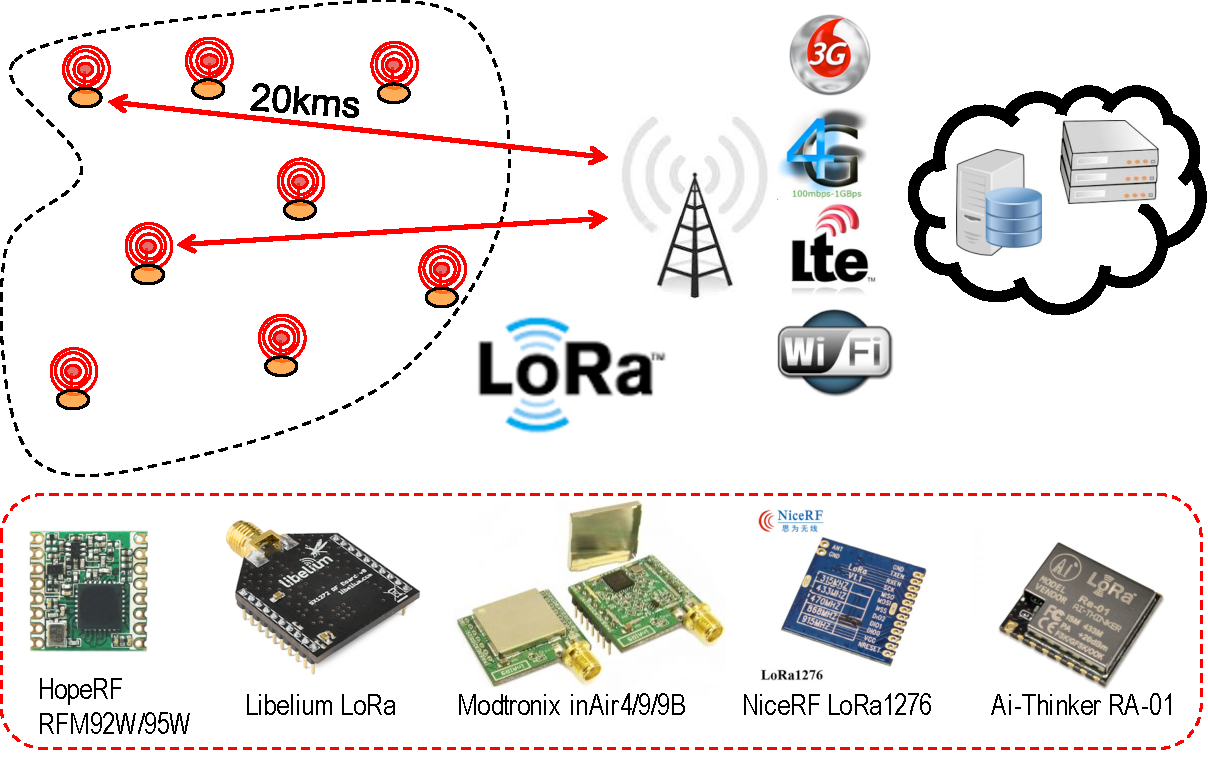
\includegraphics[width=.55\linewidth]{figures/1-hop}   
\caption{Extreme long-range application with new radio technologies}   
\label{figure-1hop}  
\end{figure} 
\end{frame}

\begin{frame}
\frametitle{Low-cost DIY IoT hardware}
 
  \begin{figure}[H]  
  \centering  
  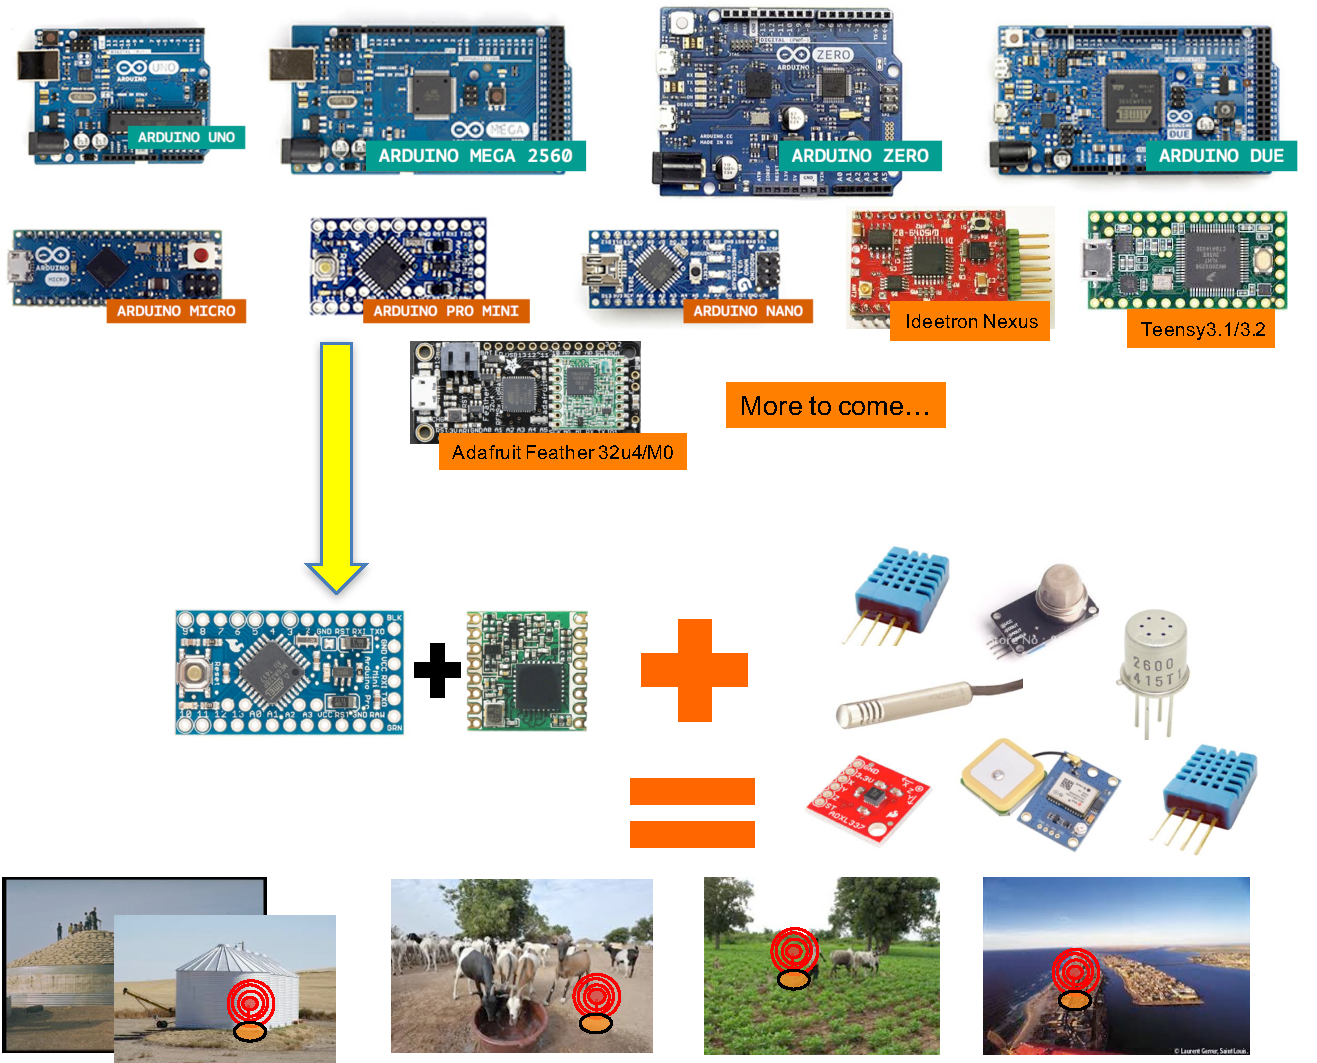
\includegraphics[width=.7\linewidth]{figures/generic-iot}   
  \caption{Generic low-cost IoT hardware}   
  \label{figure-generic-iot}  
  \end{figure} 

\end{frame}

\begin{frame}
\frametitle{Easy integration}

  \begin{figure}[H] 
  \centering  
  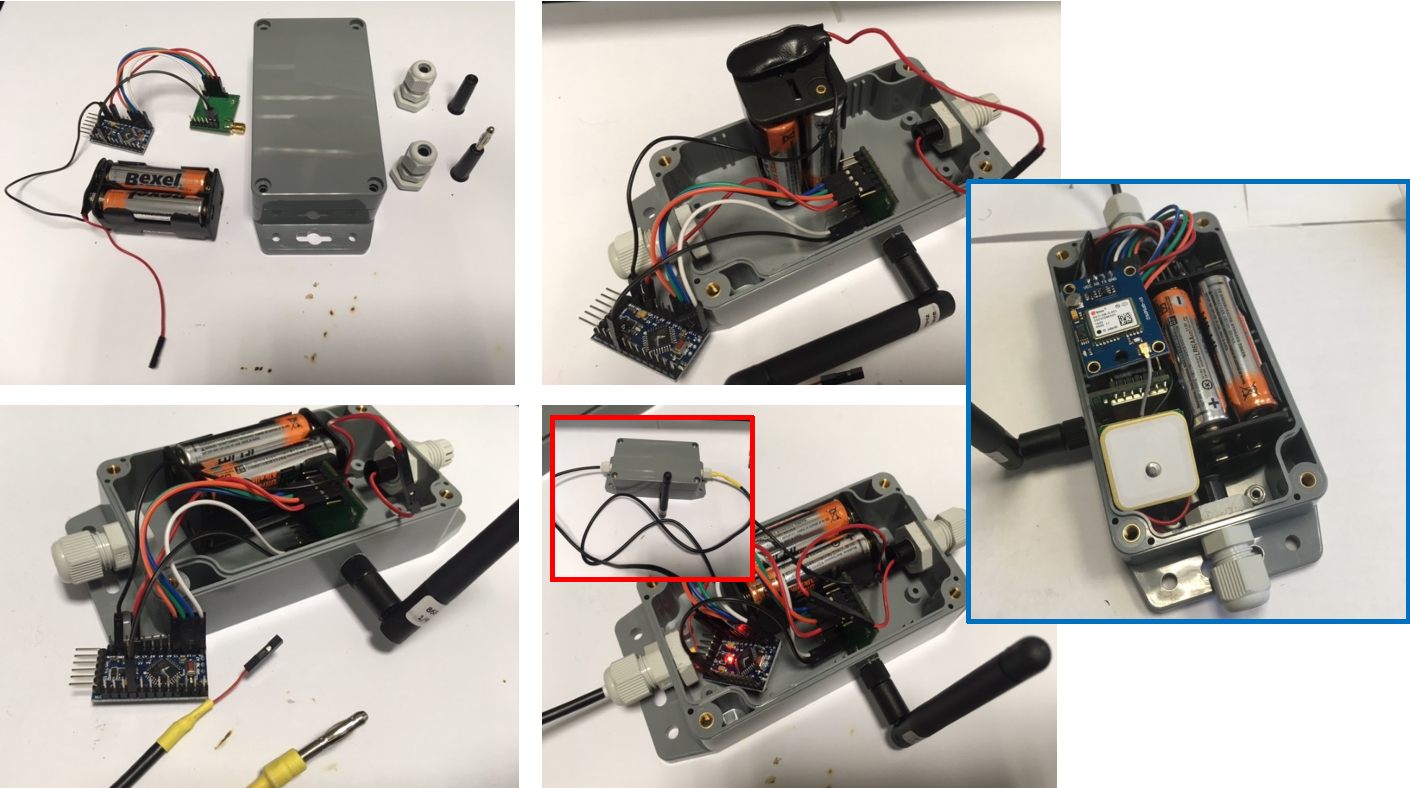
\includegraphics[width=.8\linewidth]{figures/easy-integration}   
  \caption{Easy integration with DIY approach for maximum appropriation}   
  \label{figure-easy-integration}  
  \end{figure} 

\end{frame}

\begin{frame}
\frametitle{Handling IoT data}

  \begin{figure} 
  \centering  
  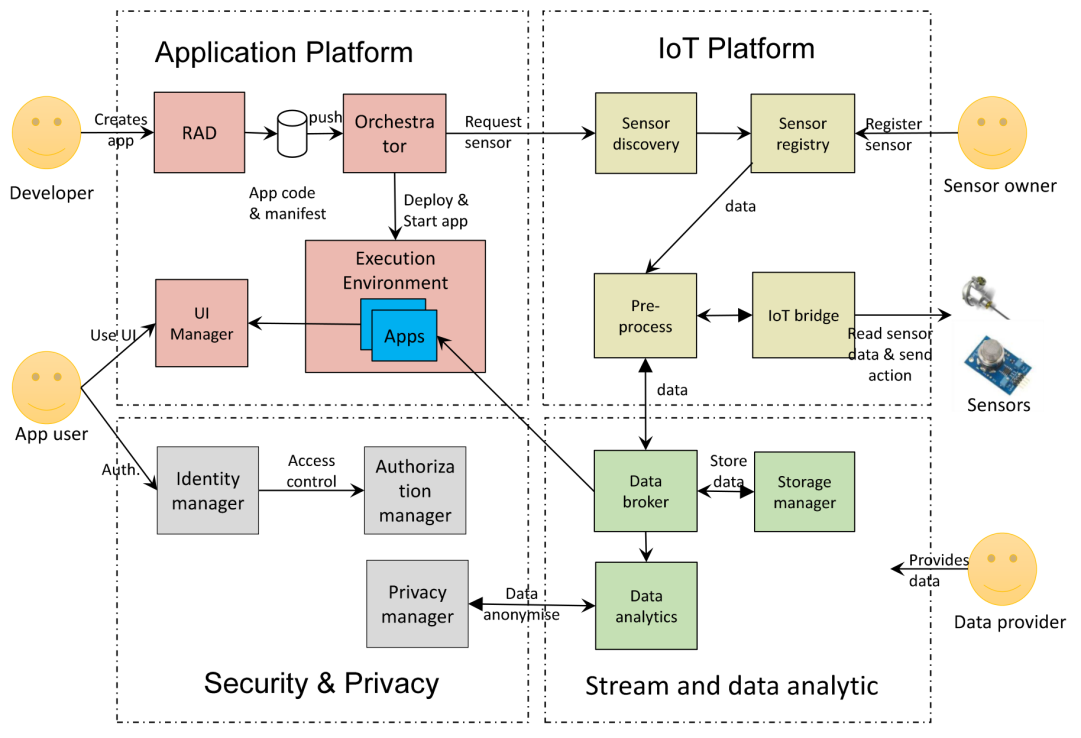
\includegraphics[width=.9\linewidth]{figures/GlobalArch}   
  \caption{IoT platform architecture}   
  \label{figure-globalarch}  
  \end{figure} 
  
\end{frame}

\section{Waziup IoT platform}

\begin{frame}
\frametitle{Architecture}

  \begin{figure}[H] 
  \centering  
  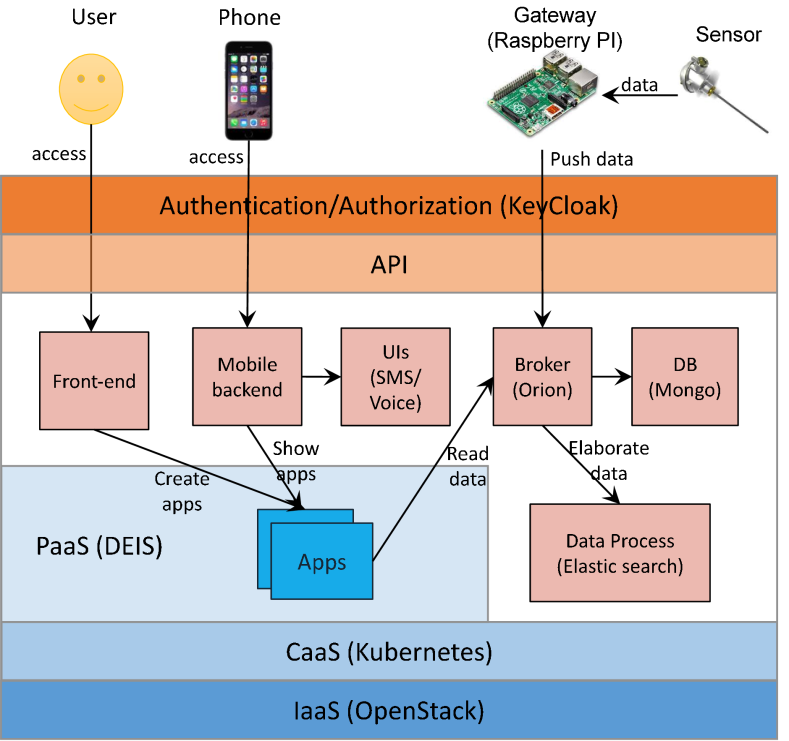
\includegraphics[width=.7\linewidth]{figures/CloudServicesArchitecture.png}   
  \caption{Global overview of WAZIUP Cloud platform, and services}
  \label{fig-implem}  
  \end{figure}

  \begin{enumerate}
    \item Infrastructure as a Service (IaaS),    
    \item Container as a Service (CaaS),    
    \item and finally Platform as a Service (PaaS).
  \end{enumerate}

\end{frame}


\begin{frame}
\frametitle{Implementation}
 
\end{frame}



\begin{frame}
\frametitle{Local and global Clouds}

  \begin{figure}[H] 
  \centering  
  \includegraphics[width=.7\linewidth]{figures/localglobalcloud}   
  \caption{Waziup local and global deployment}
  \label{fig-localglobalcloud}  
  \end{figure}
    
\end{frame}

\begin{frame}
\frametitle{Data management \& analytics}

    
\end{frame}

\begin{frame}
\frametitle{Application platform}

  \begin{figure}[H]  
  \centering  
  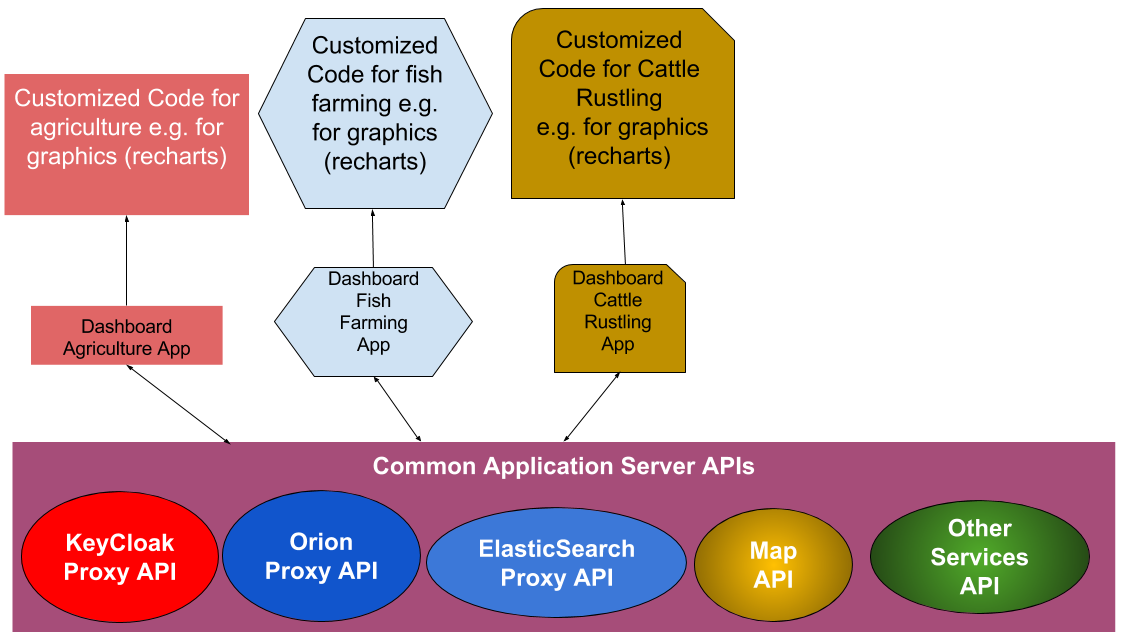
\includegraphics[width=.68\linewidth]{figures/AppArchitecture.png}   
  \caption{A global view of WAZIUP Application Template platform}
  \label{fig-app}
  \end{figure}
 
\end{frame}

\begin{frame}
\frametitle{Dashboard}

  \begin{figure}[H]  
  \centering  
  \includegraphics[width=.73\linewidth]{figures/dashboard} 
  \caption{A customized dashboard application for the soil moisture scenario}
  \label{fig-dashboard}
  \end{figure}
  
  \vspace{-1cm}
  \begin{figure}[H]  
  \centering  
  \includegraphics[width=.73\linewidth]{figures/sensor-data}
  \caption{Historical data from sensor device}
  \label{fig-sensor-data}
  \end{figure}
 
\end{frame}

\subsection{Service orchestration}


\begin{frame}
\frametitle{Service orchestration}

\end{frame}

\subsection{Security}

\begin{frame}
\frametitle{Platform security}
  
  \begin{figure}[H]
  \centering
  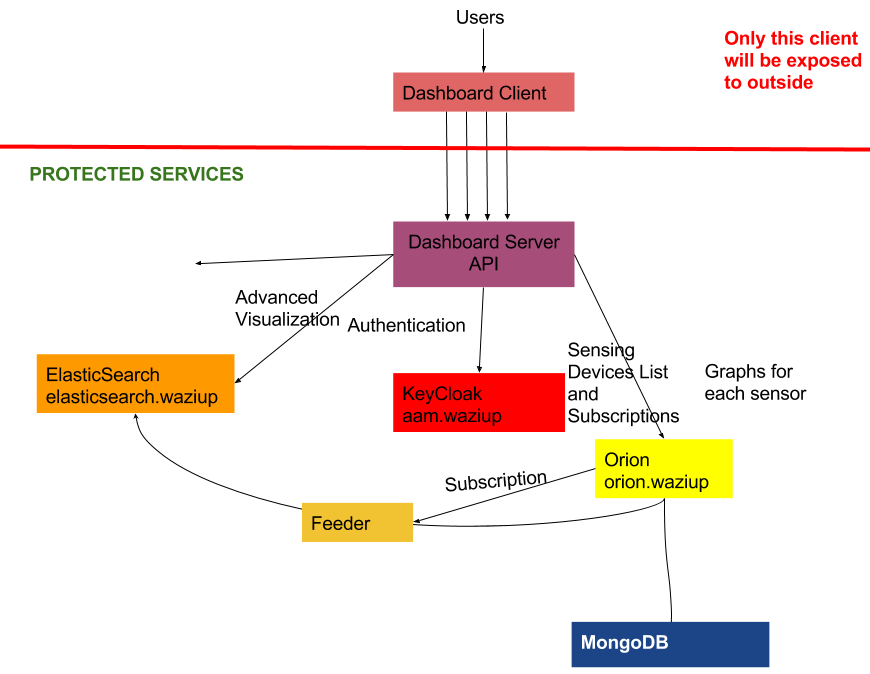
\includegraphics[width=.6\linewidth]{figures/ServicesArchitecture.png}
  \caption{Detailed view of WAZIUP Cloud platform, and services architecture}
  \label{fig-services}
  \end{figure}

  \begin{itemize}
  \item Authentication for interactive use:
  A user accesses a page (e.g. through a Dashboard web client).
  The browser sends a request to the APIs server.
  The server finds out that client has not authenticated yet and redirects the client's browser to a login screen provided by {\tt Keycloak}.
  
  
  \item Authentication for programmatic use (e.g. from a sensor gateway):
  A user generates (typically through some web-based client) an offline access refresh token.
  The token is given to a device (e.g.
  the sensor gateway) as a configuration parameter.
  When the device wants to make a request, it contacts {\tt Keycloak} and requests an access token to be generated based on the refresh token.
  
  
  \end{itemize}

\end{frame}


\section{Conclusion}

\begin{frame}
\frametitle{Conclusion}
  
With ICT technologies, developing countries can dramatically improve its productivity by enabling the rapid and cost-effective deployment of advanced and real-time monitoring.
However, deploying an IoT platform in developing countries comes with many challenges.
Among them, the most important are supporting low cost, low power, low bandwidth, and intermittent Internet.

We presented:
  \begin{itemize}
    \item Hardware
    \item software Cloud platform 
  \end{itemize}

\end{frame}


\begin{frame}
\frametitle{Acknowledgements}

The authors would like to thank the EU H2020 projects Waziup, and the Create-Net FBK research centre. \\

\end{frame}

\end{document}
